%In order to sail properly and make the most out of the wind that’s is supplied by the nature itself some data acquisition is needed. The sailing is all about this harnessing all the forces of the nature and the wind that it pushing towards you. Since there has not been any other extensive projects and measurements in this particular area the measurements have to be done in new ways. 
Since all kinds of sailboats main feature is to move completely analogue without the need of fuel or electricity, the use and optimization of surrounding forces are of foremost importance. Measuring this will provide the sailor with all the information needed to optimize the way they move and control their dinghy.

To get any kind of measurements of the dinghy, sensors are needed. As of now there are sensors measuring a wide array of items. This section will talk about these sensors; what they measure, where they were purchased, the requirements on the sensor, their features, drawbacks and also how they were implemented.
Since the sensors have to work in this particular system prototypes are made around the sensors to acquire the data.
Designs are made with the \gls{CAD} software Fusion 360\cite{cad}. The models are manufactured using a 3D printer for fast and easy development.

\subsection{Force sensors}
The function of the daggerboard is to compensate for the force that the wind is pushing on the sail which also helps to hold the dingy level in the water. The goal is to have a system that can measure the forces that pushes on the daggerboard by the water it goes through. By measuring the side forces on the board, a rough estimation of the exerted force on the sail can be made. 


\subsubsection{The implementation}
After some different solutions was suggested the final sensor and measurement method was chosen as the most prominent and clean approach. 
Important to know is that every solution is mandatory to be waterproof and sealed properly from the harsh environment that this system has as its home turf. 
With this implementation the daggerboard itself will not be disassembled or modified in any way. 
Solutions that required the sensors to be mounted on the outside or in parts that would be in danger if a crash might occur was scratched.  
Other solutions are, either way, more difficult to apply and mount or more complex.  


\subsubsection{The prototype}
To implement the gauges, a prototype is designed to show how the measurements will be made. The prototype is a bit bigger than the intended solution for this project but it's good to see how it would be constructed. The function is easy to understand. The board goes on the outside and can easily slide up and down past this steel bead. The bead itself is kept inside a small space where it can move in and out.
 
\begin{figure}[H]%look at later figures comment
\begin{center}
	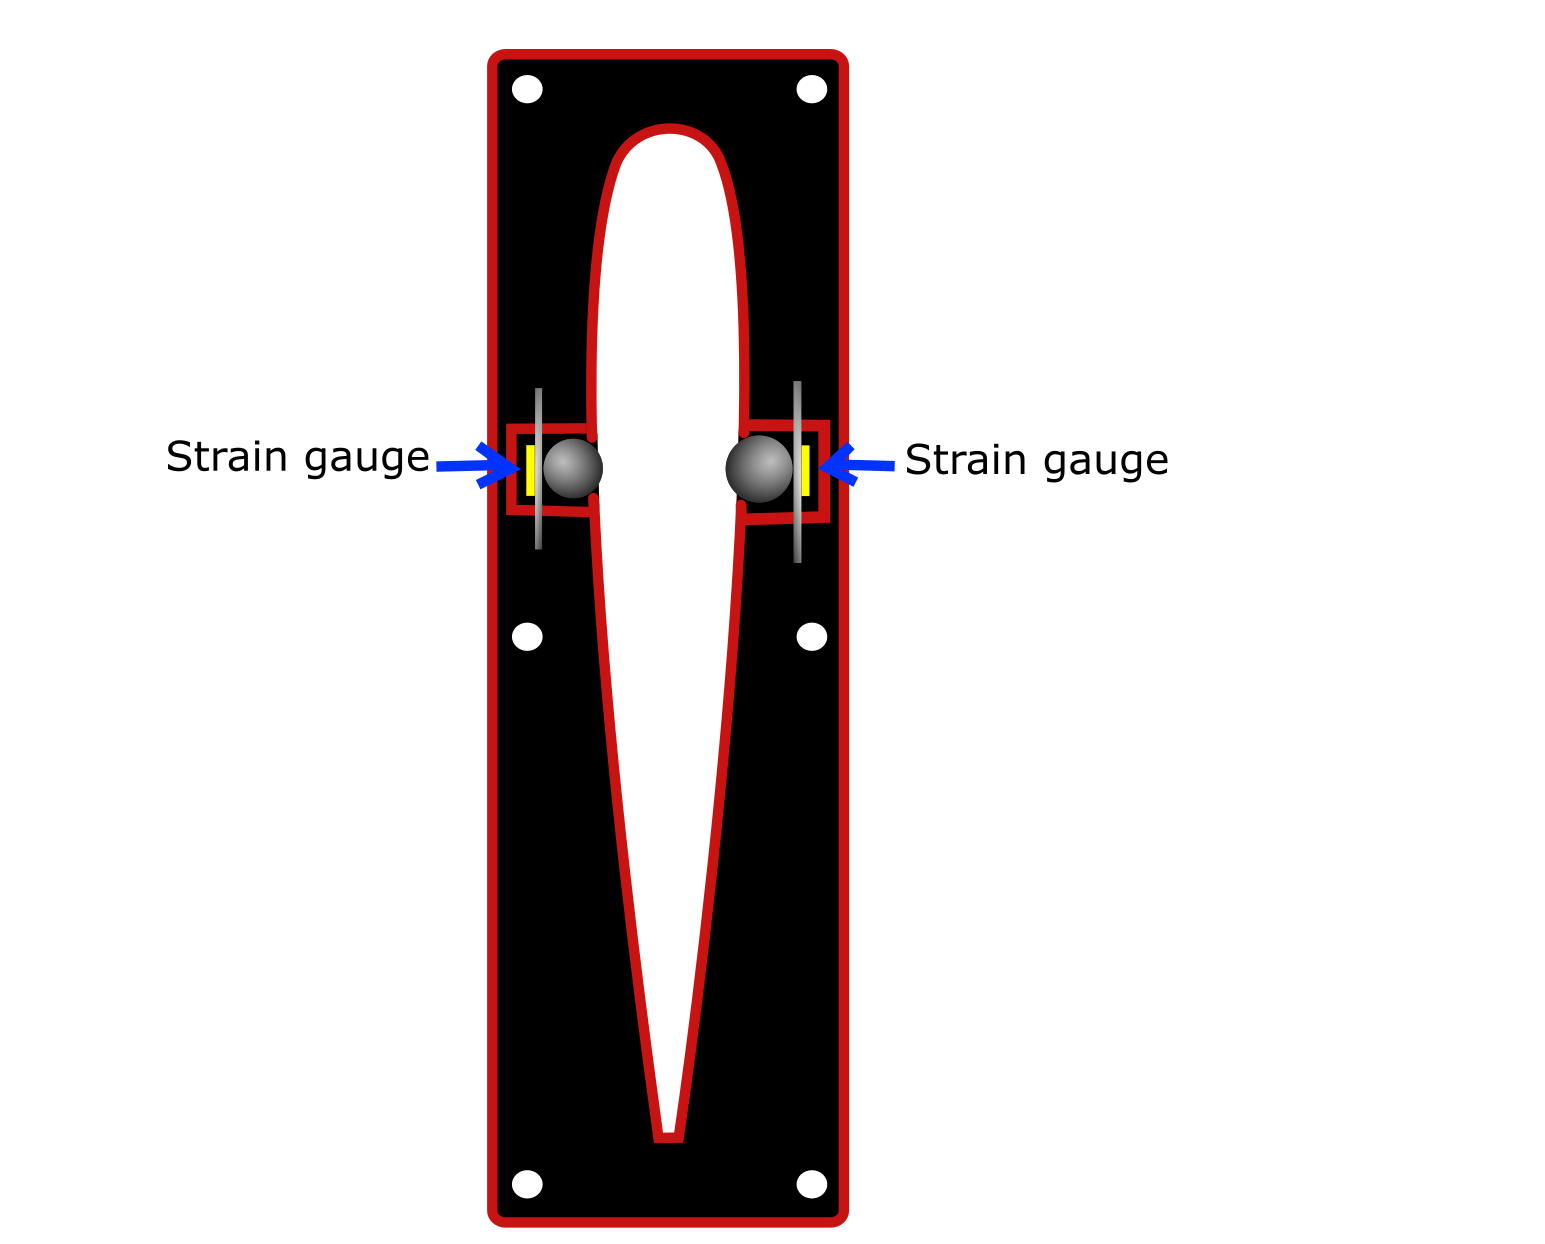
\includegraphics[width = 10cm]{Figures/Prototyp_1.png}
	\caption{Function of first prototype}
	\label{Press_sens_prot_1}
\end{center}
\end{figure}

A model of the pressure sensor was created in order to clearly show the function of this sensor and to help the thought process involved in the improving of this design.

\begin{figure}[H]%look at later figures comment
\begin{center}
	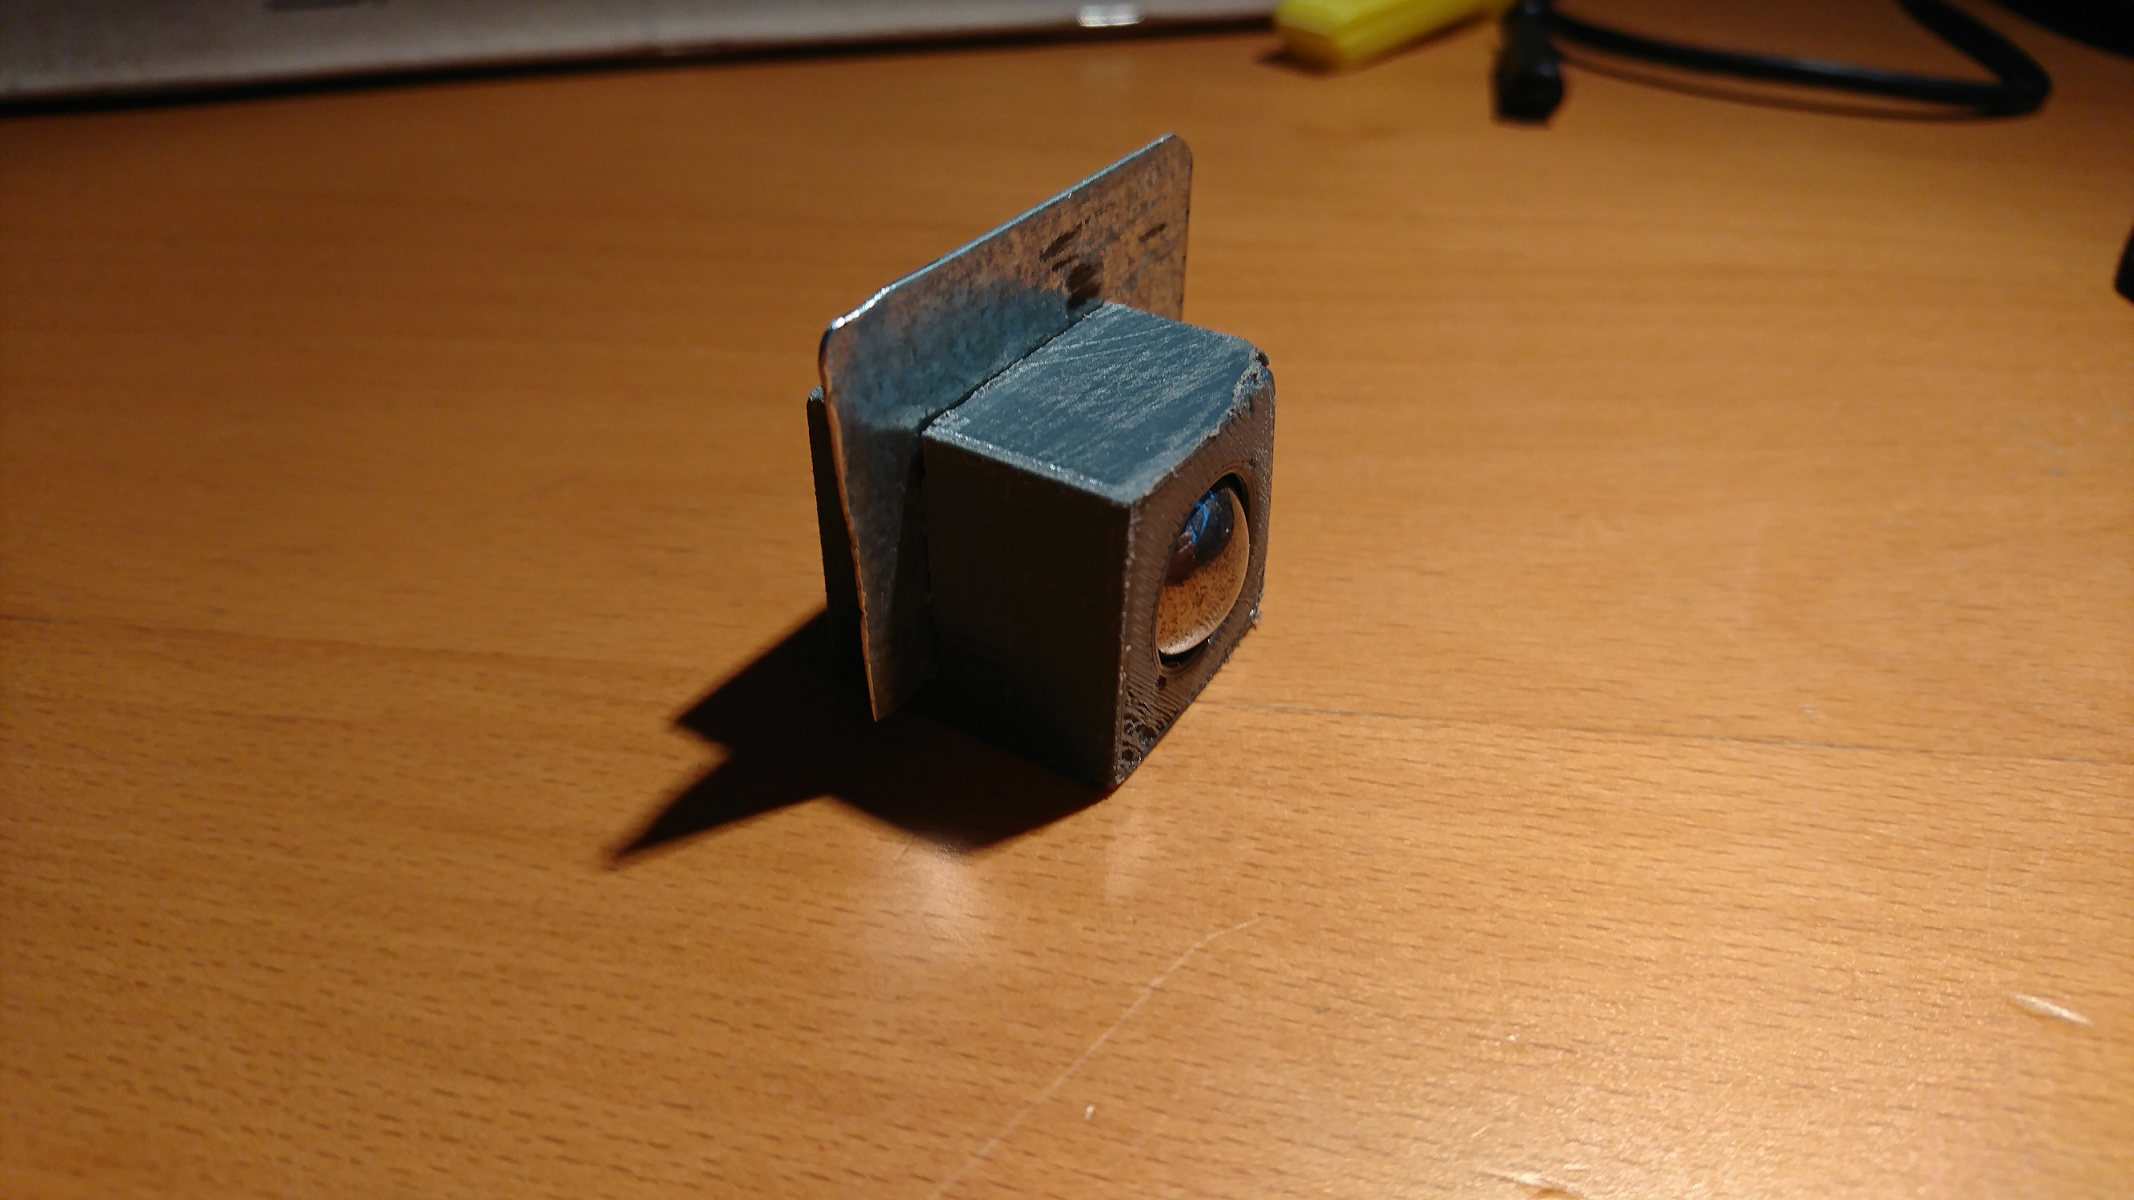
\includegraphics[width = 10cm]{Figures/Press_sens_prot_1.png}
	\caption{Function of first prototype}
	\label{Press_sens_prot_1}
\end{center}
\end{figure}

The force is measured at the back where there will be a plate. The deflection of this plate which will be the origin to the strain will be measured through strain gauges. 
The gauge itself will measure a small difference in resistance. This small difference is going to be difficult to measure without any amplifying circuit connected. With a such small signal the system might have issues with noise. Another problem is the signal might drift, and therefore make different measurements as the circuit is running. And finally, with the measured values getting amplified with a big amount the resulting signal may be off by a large amount. 

A better solution is to make some research into load cells, which is a sensor which also utilizes strain gauges to measuring forces. The difference is that the gauges are already implemented in the sensor. The difference in this prototype is instead of having a metal plate, it can be built with a piece of plastic or rubber which can deform so the force is distributed directly to the sensor. By implementing this sensor, a lot of time was saved in troubleshooting. And by having a sensor unit, the modified mounting plate will be easier to produce. 
 
\begin{figure}[H]%look at later figures comment
\begin{center}
	
\includegraphics[width = 10cm]{Figures/Press_sens_func_2.png}
	\caption{Function of second prototype}
	\label{Press_sens_prot_2}
\end{center}
\end{figure}


\subsubsection{Sensor}
The force from the board onto the mounting plate will be a considerable amount. The actual force is something that’s not known for sure. The initial assumption was that a load cell with a $90.75$ kg force range should be enough. If the sensor will be maxed out the cell it's rated for a $150\%$ overload without causing some damage to the sensor.  

The chosen sensor for this application is this part, the compression load cell called FX1901\cite{load cell}.  
From the datasheet, the voltage readings of this part could be calculated. The maximum voltage difference is calculated to be around $180mV$. 

\begin{figure}[H]%look at later figures comment
\begin{center}
	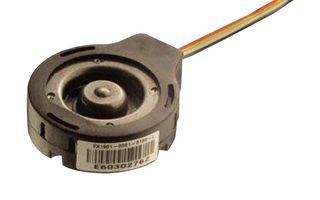
\includegraphics[width = 10cm]{Figures/Load_cell.png}
	\caption{Load cell, FX1901}
	\label{Load_cell}
\end{center}
\end{figure}


\subsection{Amplifier}
With a such small signal, an amplifier is needed to get some desired measurements. A good measurement signal to the MCU should be in the order of in between$0–3.3$ volts. Since the maximum value from the load cell is 180mV an signal of 3.3 volts is achieved by an amplification gain of around $20$.  

A suitable amplifier needs to be chosen from this implementation. Inspiration is taken from The University of Chicago\ref{UoC} in an experiment where they use this exact load cell together with an instrumental amplifier called INA125. This amplifier is somewhat more complicated and has some more features that other amplifiers.  

In the same family of instrument amplifiers, a model called INA126 is selected as a less complicated and more power efficient solution.  
This amplifier has a smaller power draw due to some simpler functions and lesser precision. But for this application it's sufficient.  
The implementation is easy and the gain can easily be determined by connection a resistor Rg between two pins on the amplifier. 

\begin{figure}[H]
\begin{center}
	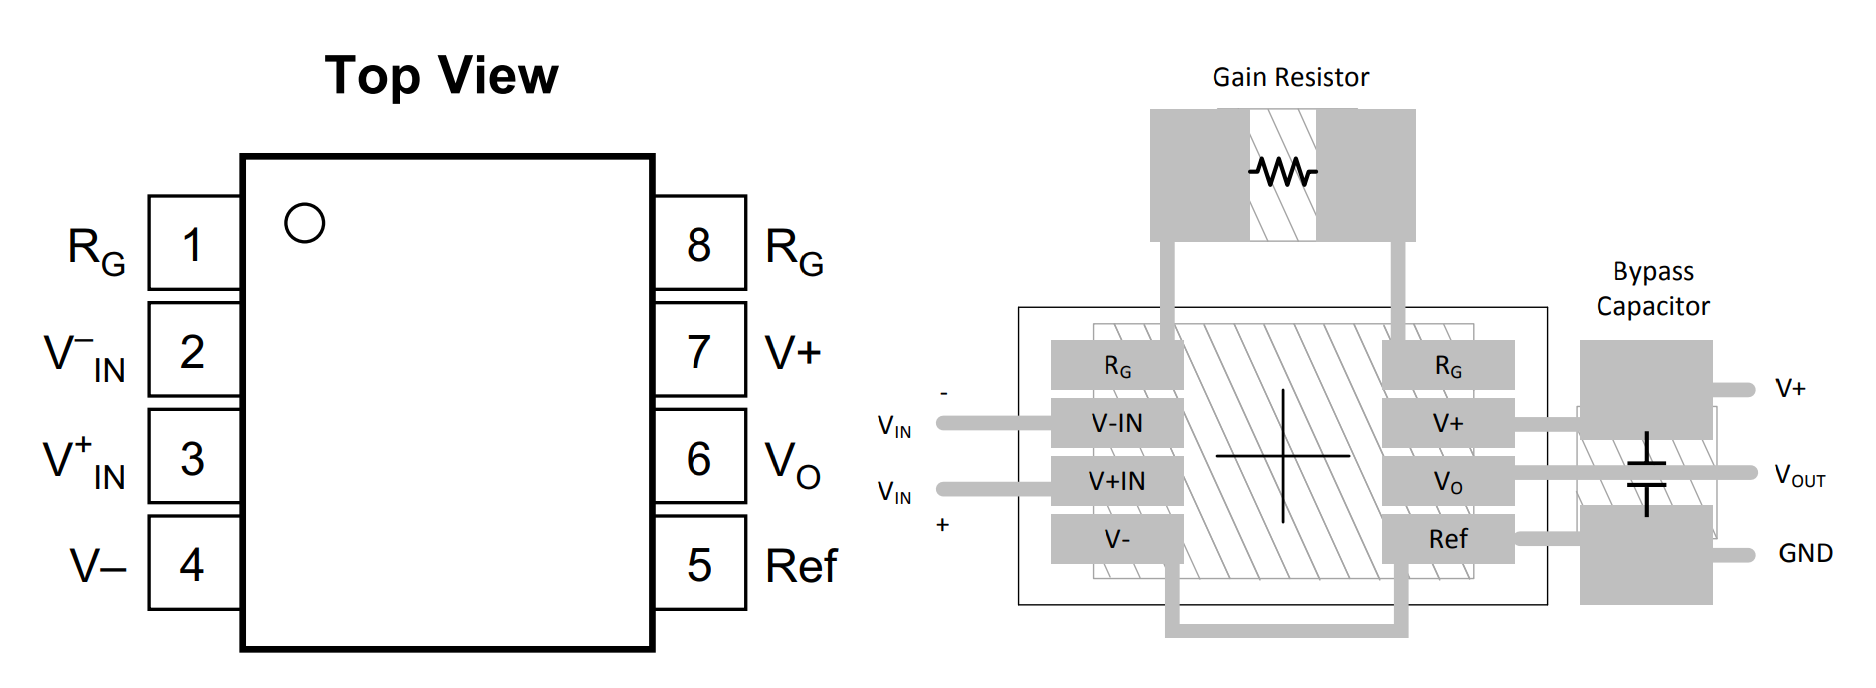
\includegraphics[width = 10cm]{Figures/INA126_pinout.png}
	\caption{Amplifier for the load cell signal}
	\label{INA126}
\end{center}
\end{figure}

The gain on this piece is easily calculated with following function.  

\begin{equation}%add a \label{labelname} to refer to this equation.
\textrm{Gain} = 5 + \frac{80~\textrm{k}\Omega}{R_G}
\end{equation}

In order to adjust the gain of the amplifier the resistor $R_G$ is set to a fixed resistor in series with a potentiometer.


\subsection{Height of centerboard sensor}
The height of the daggerboard is a crucial measurement in dinghy sailing. The daggerboard not only gives the dinghy a corresponding force to the sail, the board can also be a danger if you sail in running wind. One of the best implementations of a height sensor would be the use of a linear wire distance sensor. This sensor measures how far a wire is pulled, which gives a very accurate measurement. This solution can be totally watertight and concealed in the main centerplate. Other solutions can be to use some type of light sensor. 

\subsubsection{Sensors}
%The sensor fulfilling our requirements of both functionality and size is the following, NAME, see fig. (\ref{FIGURELABEL}). It is ..

A suitable product has been found, which is very accurate and reliable, the Micro epsilon mk30\cite{micro-epsilon-mk30}.

It's physical volume in small enough with a size of 3x5cm. As the product have some tight space constraints this can probably fit inside the case. This particular sensor is in the range of 2000kr. If no other solution works as intended this might be considered again.
The main issues might be that the height of centerboard: % That the height of the centerboard what?
One of the best implementations of a height sensor would be the use of a linear wire distance sensor. This particular sensor measures how far a wire is pulled, which gives a very accurate measurement. This solution can be completely watertight and concealed in the main centerboard.  

\begin{figure}[H]% As mentioned before, H -> tb, Refer to all figures used, use width only to /restrict/ size.
\begin{center}
	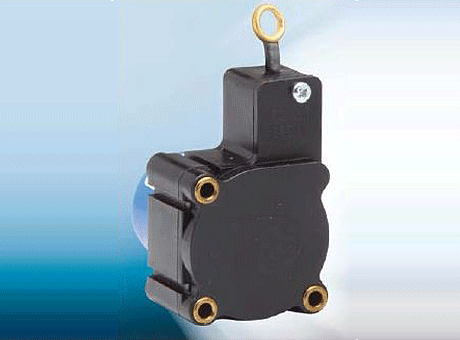
\includegraphics[width = 10cm]{Figures/microepsilon_mk30.png}
	\caption{Linear draw wire sensor, Micro epsilon MK30}
	\label{Draw_sensor}
\end{center}
\end{figure}

Light sensors have also been considered. This is implemented with the use of a plate placed on top of the dagger-board and with the light being sent up to this panel, the height can be calculated. First, we looked into some \gls{IR}-sensors. They will send the signal in a widespread which will make the distance measurement troublesome as this signal has just a small plate to bounce off.

With the use of a \gls{lidar} system, we can point our light signal at an exact spot and then get an exact measurement of the height.  
Many of the \gls{lidar} systems found was both too large and expensive to be implemented in this project.
A new product called "micro-lidar" can be used, as it is both have a small form factor and is easy to implement.
The chosen circuit is VL53L0X from Adafruit\cite{micro_lidar}. 

\begin{figure}[H]
	\centering %\centering can be used inside environments (i.e. all \begin{} here \end{}) and centers everything inside.
	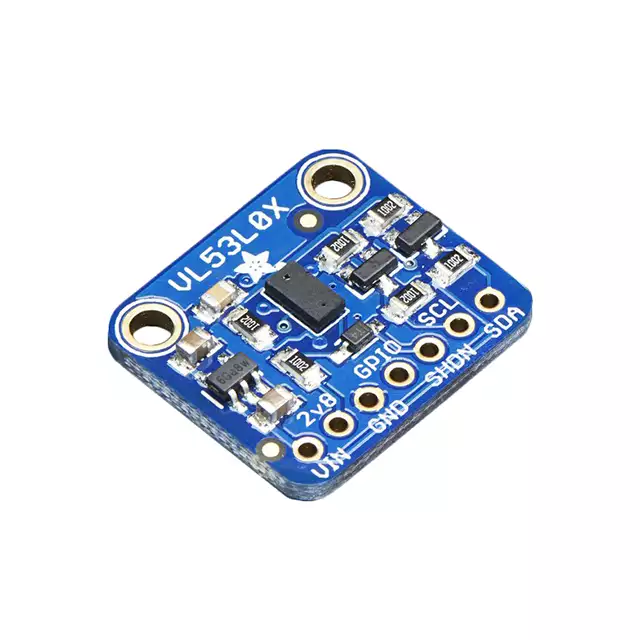
\includegraphics[width = 10cm]{Figures/Adafruit_height_sensor.png}
	\caption{Time of flight, $\mu$\gls{lidar}, distance sensor Adafruit VL53L0X}
	\label{micro_lidar}
\end{figure}

It can measure hights up one meters with great accuracy and communicates with \gls{i2c}.

By the fact that the sensor must be waterproof the signal has to go through a medium. The medium can be some type of plastic or even glass.   

All the information about this sensor when used with a cover widow can be found in the specific datasheet: “VL53L0X ranging module cover window guidelines” \ref{Tof_cover}. The maximum thickness of the cover window and the air gap between the sensor and the window is 2 mm. That’s the parameters that need to be considered. The cover window can be some type of plastic or glass. To reflect the signal a detection plate is constructed and fastened to the top of the daggerboard. This plate is level with the sensor and has a white underside for best performance of the sensor. 

\begin{figure}[H]
	\centering %\centering can be used inside environments (i.e. all \begin{} here \end{}) and centers everything inside.
	\includegraphics[width = 10cm]{Figures/height_mesure.jpg}
	\caption{Height measurement model}
	\label{height_measure}
\end{figure}


\subsubsection{Results}

The sensor works very well in the open air and can detect heights up to 1.5 meters with great accuracy. It also works well when used behind a thin plastic cover. With a 1mm thin plastic cover the maximum heigt measurement is decresed to about one meter. In the case the sensor is mounted behind a thin epoxy window witch was to thick at the beginning but was sanded down to a sutible thickness. The final window was then polished to a crystal clear finish for the best measurements. The measurement is heavily dependent on the the finish of the window, if there is small inperfections on the window such as scratch the sensor can't take measurements.

As there will always be water around and on the center plate the light that is sent might get directed "wrong" if there are only some small water droplets in between the sensor and the panel that we want to reflect our light on.  

This system can definitively be improved in the future with either a completely different measurement system or with a better implementation of the window cover. The window cover probably would work better if the cover was molded in a convex form, which could lead off the water droplets formed on the window surface. This in cooperation with a surface finish that repels water, such as a hydrophobic coating would be a great solution. 


